\documentclass[12pt]{article}
\usepackage[spanish, mexico]{babel}
\usepackage{dsfont}
\usepackage{amsmath}
\usepackage{amsthm}
\usepackage{amsfonts}
\usepackage{IEEEtrantools}
\usepackage{caption}
\usepackage{listings}
\usepackage{graphicx}
\graphicspath{ {images/} }
\pagestyle{headings}
\begin{document}
\title{Apuntes sobre Álgebra Superior II}
\author{Elmer Ortega}
\maketitle
\section*{El campo de los complejos}
%¿Qué es un \textbf{Anillo}?
\noindent Un conjunto $A$ con las operaciones definidas suma ($+$) y producto ($\cdot$)
\begin{center}
    $\langle A, +, \cdot \rangle$
\end{center}
se llama \textbf{Anillo} si cumple las siguientes 8 propiedades:
\begin{enumerate}
    \item \textbf{La suma cierra}  (cerradura) : 
    \begin{center}
        $\forall a,b \in A,  a+b\in A$
    \end{center}
    \item \textbf{El producto cierra}  (cerradura) : 
    \begin{center}
        $\forall a,b \in A,  a \cdot b\in A$
    \end{center}
    \item \textbf{Neutro aditivo} : 
    \begin{center}
        $\exists{ } 0 \in A$ \text{tal que} $\forall a \in A, a+(0)=(0)+a=a$
    \end{center}
    \item \textbf{Inverso aditivo} : 
    \begin{center}
        $\exists -a \in A$ \text{tal que} $\forall a \in A, a+(-a)=(-a)+a=0$
    \end{center}
    \item \textbf{Comutatividad de la suma} : 
    \begin{center}
        $\forall a,b \in A,  a+b=b+a$
    \end{center}
    \item \textbf{Asociatividad de la suma} : 
    \begin{center}
        $\forall a,b,c \in A, (a+b)+c=a+(b+c)$
    \end{center}
    \item \textbf{Asociatividad del producto} : 
    \begin{center}
        $\forall a,b,c \in A, (a\cdot b)\cdot c = a \cdot (b \cdot c)$
    \end{center}
    \newpage
    \item \textbf{Distributividad$\dots$} \newline 
        $\forall a,b,c \in A,$
        \begin{itemize}
            \item \textbf{por la izquierda:} $a\cdot( b + c) = ab+ac$
            \item \textbf{por la derecha:}  $( b + c)\cdot a = ba+ca$
        \end{itemize}
    Si se cumple la siguiente condición, entonces el anillo $\langle A,+,\cdot\rangle$ se llamará \textquotedblleft Anillo con 1\textquotedblright.
    \item \textbf{Neutro multiplicativo}
    \begin{center}
        $\exists{} 1, \forall a \in A, 1a=a1=a$
    \end{center}
    Si se cumple la condición de \textbf{producto conmutativo} el anillo $\langle  A,+,\cdot \rangle$ se llamará \textquotedblleft anillo conmutativo \textquotedblright. 
    \begin{center}
        $\forall a,b\in A, a\cdot b = b \cdot a$
    \end{center}
     \textbf{Ejemplo:} $\langle  \mathbb{Z}, +, \cdot \rangle$ es un \textquotedblleft anillo conmutativo con 1 \textquotedblright.

    \textbf{Def.} Un campo $\langle K, +, \cdot \rangle$ es un anillo conmutativo con 1 que además cumple:
    \item \textbf{Existencia del inverso multiplicativo}:
    \begin{center}
        $\forall a \in A, a\not = 0, \exists a^{-1}\in A \text{ tal que } a\cdot a^{-1}=a^{-1}\cdot a =1$
    \end{center}
    \textbf{Ejemplo:} $\langle \mathbb{Q}, +, \cdot \rangle$ es un anillo conmutativo con 1 en el que, además, si \newline
    \begin{center}
    $\forall\dfrac{a}{b}\in\mathbb{Q}$ \^{} $ a\not=0 ,\exists \dfrac{b}{a} \in \mathbb{Q}$ \^{} $\left( \dfrac{a}{b} \right)\left( \dfrac{b}{a} \right)=1$
    \end{center}
    entonces $\langle \mathbb{Q}, +, \cdot \rangle$ es un campo.
\end{enumerate}
\newpage
\subsection*{¿Cómo surge los números $\mathbb{C}$omplejos?}
Cuando construirmos conjuntos de números lo hacemos para solucionar problemas que nos complican la vida.
 El primer problema de la humanidad fue contar colecciones de objetos por lo que surgio la noción de los números 
$\mathbb{N}$aturales $\left\{1,2,3 \dots \right\} $.
\newline
\newline
Cuando quisimos resolver $x+4=0$ no encontramos un $x\in\mathbb{N}$ que la cumpla, así que surgió la noción de los enteros
$\mathbb{Z} = \left\{\dots-2,-1,0,1,2\dots\right\}$.
\newline
\newline
Ahora, quisimos resolver $2x+3=0$ no encontramos un $x\in\mathbb{Z}$ que la cumpla, así que surgió la noción de los racionales
$\mathbb{Q} = \left\{\dfrac{a}{b}|a,b\in\mathbb{Z}, b\not=0\right\}$.
\newline
\newline
Después, quisimos resolver $x^2-=0$ no encontramos un $x\in\mathbb{Q}$ que la cumpla, así que surgió la noción de los irraciones,
aquellos ${\mathbb {I} :=\mathbb {R} \backslash \mathbb {Q} =\{x\in \mathbb {R} |x\notin \mathbb {Q} \}}$,
y números reales $\mathbb{R} = \mathbb{Q}\cup\mathbb{I}$.
\newline
\newline
Y, por último, surgió la ecuación $x^2+1=0$, el famoso conjunto de los números $\mathbb{C}$ omplejos.
\newline
\newline
\textbf{Definición: }Se define el número imaginario como $i=\sqrt{-1}$
\newline
\newline
\textbf{Definición: }Se define un número $w\in\mathbb{C}$ si cumple que $w=a+bi$ donde $a,b\in\mathbb{R}$
\newline
\newline
\textbf{Definición: } Sea $w=a+bi \in\mathbb{C}$, se define la función de parte real de $w$ como $Re(w)=a$
\newline
\newline
\textbf{Definición: } Sea $w=a+bi \in\mathbb{C}$, se define la función de parte imaginaria de $w$ como $Im(w)=b$
\newline

\noindent \textbf{Exponentes de }$i$ :
\begin{center}
    $i^{4k}=1\rightarrow$ 
    $i^{4k+1}=i\rightarrow$
    $i^{4k+2}=-1\rightarrow$
    $i^{4k+3}=-i$     
\end{center}
\newpage
\noindent \textbf{Definimos en } $\mathbb{C}$:\newline
$\bullet \textbf{ la suma} +$ como $w=a+bi,\text{ }z=c+di, \Rightarrow w+z=(a+c)+(b+d)i$ \newline
$\bullet \textbf{ el producto} \*$ como $w=a+bi,\text{ }z=c+di, \Rightarrow$ \newline
$w*z=(a+bi)(c+di)=ac+adi+bci+bdi^2=(ac-bd)+(ad+bc)i$\newline
$\bullet \textbf{ el neutro aditivo} $ como $0=0+0i$\newline
$\bullet \textbf{ el neutro multiplicativo} $ como $1=1+0i$\newline
$\bullet \textbf{ el inverso multiplicativo} $ como:\newline
Sea $w=a+bi \Rightarrow w^{-1}=\dfrac{a}{a^2+b^2}+\dfrac{-b}{a^2+b^2}i\text{ con } a$ y $b\not=0$\newline
Corroborando las 10 preposiciones mencionadas antes podemos comprobar que $\langle\mathbb{C}, +,\cdot\rangle$ es un \textbf{campo}.\newline
*\textbf{Nota importante: } $\mathbb{C}$ no es un campo ordenada, es decir, no tiene sentido la comparación
de $z_1,z_2\in \mathbb{C}$ tal que $z_1 < z_2$\newline
\subsection*{Conjugado de $z$}
\noindent \textbf{Definición: }Para cada $z\in\mathbb{C}, z=a+bi$, entonces se denomina
\textbf{conjugado de }$z$ a $a-bi$ y se denota $\bar{z}$
\newline
\subsection*{Propiedades del conjugado de un complejo}
Sea $z=a+bi,w\in\mathbb{C}$
\begin{enumerate}
    \item $z \cdot \bar{z}=a^2+b^2$
    \item $\bar{z+w}=\bar{z}+\bar{w}$
    \item $\bar{z\cdot w}=\bar{z}\cdot\bar{w}$
    \item $\bar{\bar{z}}=z$
    \item $\bar{\dfrac{z}{w}}=\dfrac{\bar{z}}{\bar{w}}$
    \item $Re(z)=\dfrac{z+\bar{z}}{2}$
    \item $Im(z)=\dfrac{z-\bar{z}}{2i}$
\end{enumerate}
\subsection*{Representación geométrica y polar de los $\mathbb{C}$ omplejos}
\noindent\textbf{Representación geométrica en $\mathbb{R}^2$}
\begin{center}
    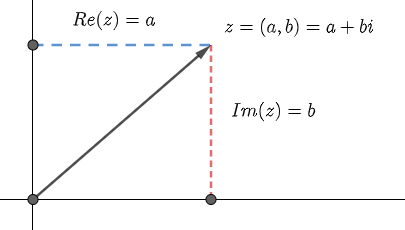
\includegraphics{imaginariosGeo.png}
\end{center}
\noindent\textbf{Representación polar en $\mathbb{R}^2$}
\begin{center}
    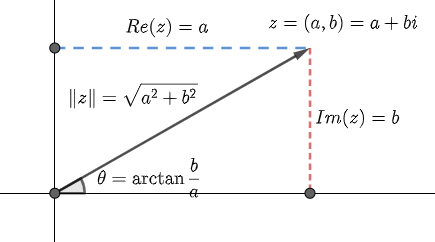
\includegraphics{imaginariosGeo1.png}
\end{center}
\newpage
\subsection*{Conversión de las representaciones}
\noindent\textbf{Pasar a forma geométrica a polar}
\begin{center}
    $\|z\|=\sqrt{a^2+b^2}$, $\theta=\arctan{\left(\dfrac{b}{a}\right)}$    
\end{center}
\begin{center}
    $z=\|z\|(\cos{\theta}+i\sin{\theta})$
\end{center}
\textbf{Pasar a forma polar a geométrica}
\begin{center}
    $a=\|z\|\cos{\theta}$, $b=\|z\|\sin{\theta}$
\end{center}
\begin{center}
    $z=a+bi$
\end{center}
\end{document}
